The Fabry-Perot cavity comes in various constellations, but will mainly be discussing the plane-parallel, mainly for theory, or the hemispherical, which is in our current experimental setup. A stable cavity must satisfy the stability condistion

\begin{equation}
0 \leq \left(1 - \frac{L}{R_1}\right)\left(1 - \frac{L}{R_2}\right) \leq 1
\end{equation}

where $L$ is the cavity length and $R_{1,2}$ the radius of curvature of the mirrors.

The laser intensity profile has a Gaussian distribution $I(r, z) \propto e^{\frac{-2r^2}{w(z)^2}}$, since the transverse electric field distribution is well approximated by a Gaussian profile. Here $r$ is the radial distance from the center axis of the beam, $w(z) = w_0\sqrt{1 + z_R^2/z^2}$ is the beam waist size as function of longitudinal propagation direction. It can be thought of as the wave fronts no longer are plane waves, but now has radius of curvature $R(z) = z + z_R^2/z$, where $z_R = \pi w_0^2/\lambda$ is the Rayleigh range and $w_0$ is the minimum waist radius. Gaussian beam is a solution of the paraxial form of the Helmholtz equation and is crucial knowledge for working with optics.

\begin{figure}[H]
\centering
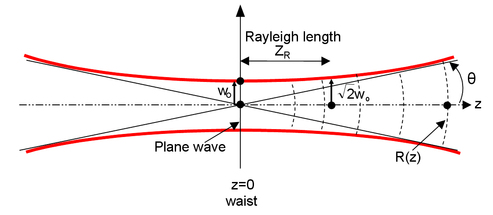
\includegraphics[scale=0.8]{Gaussian_beam.png}
\caption{Bla bla}
\label{fig:gaussian_beam}
\end{figure}

Introducing transverse modes in a cavity

\begin{figure}[H]
\centering
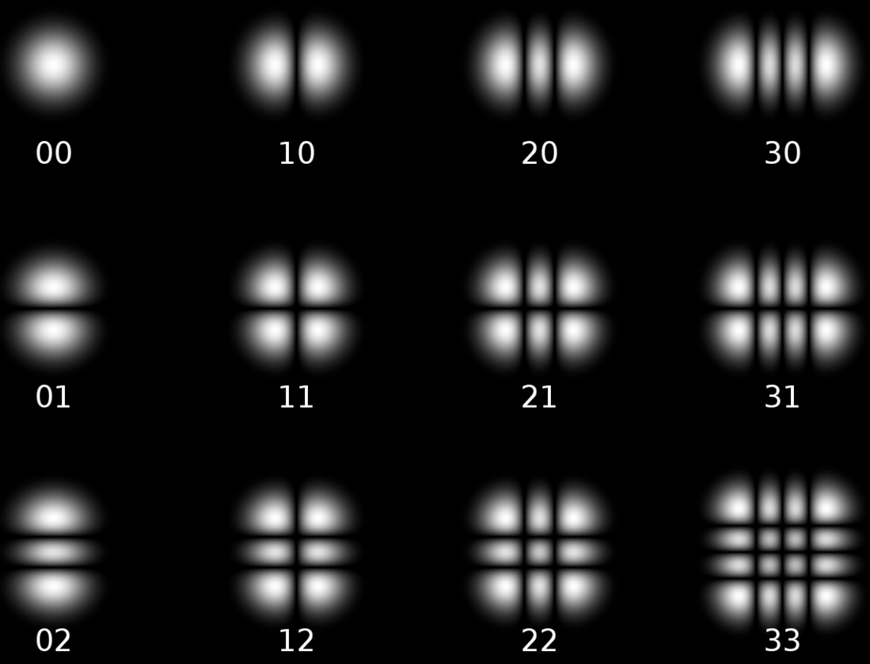
\includegraphics[scale=0.2]{Hermite_gaussian.png}
\caption{Bla bla}
\label{fig:hermite_modes}
\end{figure}